\section{Durchführung}
\label{sec:Durchführung}

\subsection{Filterkurve des Selektivverstärkers}


Hier wird die Güte des Selektivverstärkers bestimmt. Es wird mit einem Millivoltmeter
in $1 \;\mathrm{kHz}$
Schritten die Ausgangsspannung bei einer generierten Sinusspannung mit Frequenzen 
von $\nu = 20 \; \mathrm{kHz}$ bis $\nu = 40 \; \mathrm{kHz}$ gemessen. \\
Störspannungen werden durch einen Bandpass herausgefiltert
und die gesuchte Brückenspannung wird zehnfach linear verstärkt.\\
\begin{figure}
    \centering
    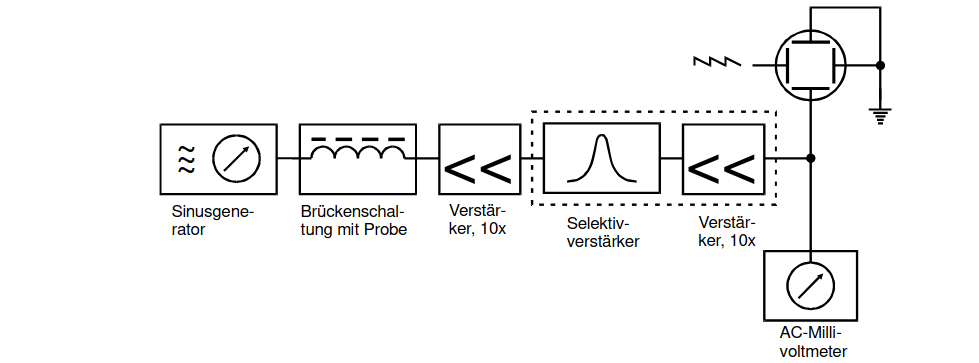
\includegraphics[width=\textwidth]{content/Aufbau.png}
    \caption{Schematischer Aufbau des Experimentes.\cite{sample}}
    \label{fig:schematisch}
\end{figure}


\subsection{Bestimmung der Suszeptibilitäten}

\begin{figure} [H]
    \centering
    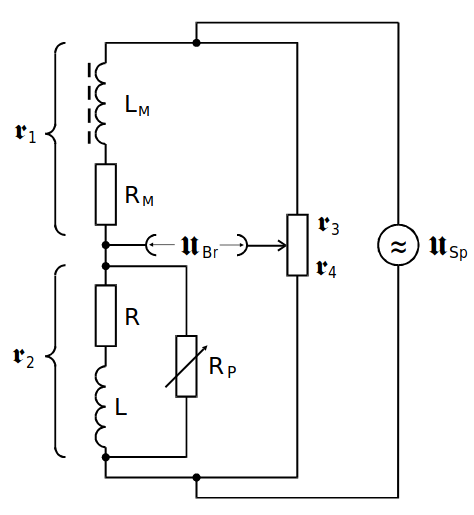
\includegraphics[width=\textwidth]{content/bild1.png}
    \caption{Brückenschaltung zur Suszeptibilitätsmessung [1]}
    \label{fig:plot1}
  \end{figure}

Zur Messung der Suszeptibilitäten wird der Sinusgenerator auf die Frequenz
eingestellt, bei der das Maximum des Selektivverstärkers liegt.\\
Er wird mit der \autoref{fig:plot1} abgebildeten Brückenschaltung verbunden, deren Ausgangsspannung zehnfach linear vorverstärkt 
wird. \\
Vor jeder Messung mit einer Probe wird die Brückenspannung ohne Probe abgeglichen, 
indem die Widerstände R$_3$ und R$_4$ so eingeregelt werden, dass die gemessene Brückenspannung minimal wird.
Es werden Spannung sowie Widerstand notiert. \\
Dann wird die Probe in die Spule eingeführt und erneut die Widerstände zwecks Spanungsminimum reguliert und 
Widerstand und Spannung notiert.\\
Da die Suszeptibilität temperaturabhängig ist, sollten die Proben Raumtemperatur haben. Deswegen ist langes in der Hand Halten zu vermeiden.\\

Dieses Verfahren wird mit drei unterschiedlichen Proben seltener Erd-Oxide, $\symup{Dy_2O_3}$, $\symup{C_6O_{12}Pr_2}$, 
$\symup{Gd_2O_3}$ und $\symup{Nd_2O_3}$, durchgeführt und jeweils drei mal wiederholt.\\
Zum Schluss werden die Massen der Proben abgelesen und deren Maße mit einem Lineal bestimmt.\\